\clearpage
\begin{explanationbox}
\textbf{一、先从初中三角形面积出发：顶点切线是最简单的模型。}

\begin{center}
% 几何准确：a=1.8,b=1.1; P=(a,0); A=(a,b); B=(a,-b)
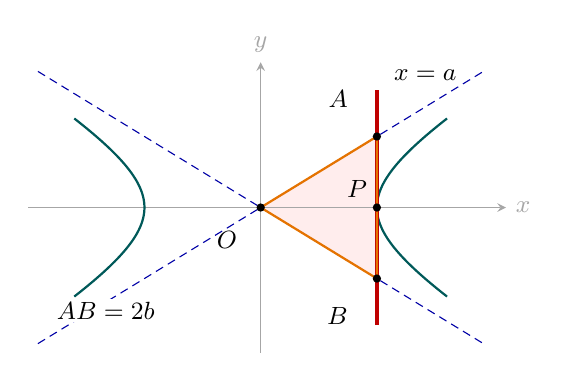
\begin{tikzpicture}[x=0.82cm,y=0.82cm,>=stealth,
  every node/.style={font=\small}]
\def\aa{1.8}\def\bb{1.1}
\coordinate (O) at (0,0); \coordinate (P) at (\aa,0);
\coordinate (A) at (\aa,\bb); \coordinate (B) at (\aa,-\bb);
\fill[red!7] (O)--(A)--(B)--cycle;
\draw[gray!70,->] (-3.6,0)--(3.8,0) node[right] {$x$};
\draw[gray!70,->] (0,-2.25)--(0,2.25) node[above] {$y$};
\draw[densely dashed,blue!65!black] (-3.45,-2.108)--(3.45,2.108);
\draw[densely dashed,blue!65!black] (-3.45,2.108)--(3.45,-2.108);
\draw[teal!70!black,thick,domain=-1.05:1.05,samples=80,variable=\t]
 plot ({1.8/2*(exp(\t)+exp(-\t))},{1.1/2*(exp(\t)-exp(-\t))});
\draw[teal!70!black,thick,domain=-1.05:1.05,samples=80,variable=\t]
 plot ({-1.8/2*(exp(\t)+exp(-\t))},{1.1/2*(exp(\t)-exp(-\t))});
\draw[red!75!black,ultra thick] (\aa,-1.82)--(\aa,1.82);
\draw[orange!90!black,thick] (O)--(A)--(B)--cycle;
\fill (O) circle(1.5pt) node[below left=5pt] {$O$};
\fill (P) circle(1.5pt) node[above left] {$P$};
\fill (A) circle(1.5pt) node[above left=7pt] {$A$};
\fill (B) circle(1.5pt) node[below left=7pt] {$B$};
\node[align=left,fill=white,inner sep=1pt] at (-2.4,-1.6) {$AB=2b$};
\node[align=left,fill=white,inner sep=1pt] at (2.55,2.05) {$x=a$};
\end{tikzpicture}

\end{center}
在右顶点 $P=(a,0)$ 处，切线是 $x=a$；渐近线上的交点为
$A=(a,b),\ B=(a,-b)$。这时 $AB=2b$，而 $O$ 到直线 $AB$
的垂距是 $a$：
\[
S_{\triangle AOB}=\frac12\underbrace{(2b)}_{\text{底边}}
\underbrace{a}_{\text{高}}=ab.
\]
\textbf{问题：}换到非顶点以后，$AB$ 会倾斜，底和高都改变。
为什么面积还能是 $ab$？\emph{不能把顶点的计算当作一般证明。}

\medskip
\textbf{二、用一个具体数字观察``一长一短''。}

取 $a=3,b=2$，右顶点对应
$A=(3,2)$、$B=(3,-2)$。如果沿两条渐近线改成
\[
A=(6,4)=2(3,2),\qquad
B=\left(\frac32,-1\right)=\frac12(3,-2),
\]
那么一边的长度变成原来的 $2$ 倍，另一边变成 $1/2$ 倍。
$OA\cdot OB$ 不变；且两条渐近线的\textbf{夹角不变}，面积也应不变。
注意此时中点为
\[
P=\left(\frac{6+3/2}{2},\frac{4-1}{2}\right)
=\left(\frac{15}{4},\frac32\right),\quad
\frac{(15/4)^2}{9}-\frac{(3/2)^2}{4}=1.
\]
这个 $P$ 的确位于双曲线上；下文将证明 $AB$ 正好是它的切线。
这一步是从\emph{现象}走向\emph{一般规律}的关键。


\medskip
\pagebreak\noindent\textbf{三、为何恰好是倒数而非任意伸缩？}

把渐近线上的点写成
\[
A=(ar,br),\qquad B=(as,-bs),\quad r,s\ne0.
\]
若 $P$ 是 $AB$ 中点，则
$P=(a(r+s)/2,b(r-s)/2)$。由于 $P\in H$，
\[
\underbrace{\frac{(r+s)^2}{4}-\frac{(r-s)^2}{4}}_{\text{平方差：展开后只剩 }rs}
=rs=1.
\]
因此 $s=1/r$。\textbf{记住的是关系 $rs=1$，不是记一个神秘的 $1/r$。}
注意：这里先用中点性质\emph{解释规律}，中点性质会在证明部分先独立证明，
不能仅凭图把它当成已知。

\begin{center}
% 几何准确：a=1.8,b=1.1, 参数 t=0.64;
% P=(a cosh t,b sinh t); A=(a e^t,b e^t); B=(a e^{-t},-b e^{-t}).
% P=(A+B)/2, OA*OB=a^2+b^2, S_OAB=ab
\begin{tikzpicture}[x=0.82cm,y=0.82cm,>=stealth,
  every node/.style={font=\small}]
\def\aa{1.8}\def\bb{1.1}\def\tt{0.64}
\pgfmathsetmacro{\XAA}{\aa*exp(\tt)}
\pgfmathsetmacro{\YAA}{\bb*exp(\tt)}
\pgfmathsetmacro{\XBB}{\aa*exp(-\tt)}
\pgfmathsetmacro{\YBB}{-\bb*exp(-\tt)}
\pgfmathsetmacro{\XPP}{(\XAA+\XBB)/2}
\pgfmathsetmacro{\YPP}{(\YAA+\YBB)/2}
\coordinate (O) at (0,0); \coordinate (P) at (\XPP,\YPP);
\coordinate (A) at (\XAA,\YAA); \coordinate (B) at (\XBB,\YBB);
\fill[red!7] (O)--(A)--(B)--cycle;
\draw[gray!70,->] (-3.6,0)--(4.25,0) node[right] {$x$};
\draw[gray!70,->] (0,-2.25)--(0,2.35) node[above] {$y$};
\draw[densely dashed,blue!65!black] (-3.45,-2.108)--(3.85,2.353);
\draw[densely dashed,blue!65!black] (-3.45,2.108)--(3.85,-2.353);
\draw[teal!70!black,thick,domain=-1.08:1.08,samples=80,variable=\t]
 plot ({1.8/2*(exp(\t)+exp(-\t))},{1.1/2*(exp(\t)-exp(-\t))});
\draw[teal!70!black,thick,domain=-1.08:1.08,samples=80,variable=\t]
 plot ({-1.8/2*(exp(\t)+exp(-\t))},{1.1/2*(exp(\t)-exp(-\t))});
\draw[red!75!black,ultra thick] ($(B)!-0.28!(A)$)--($(A)!-0.25!(B)$);
\draw[orange!90!black,thick] (O)--(A)--(B)--cycle;
\fill (O) circle(1.5pt) node[below left=5pt] {$O$};
\fill (P) circle(1.5pt) node[left=4pt,yshift=-5pt] {$P$};
\fill (A) circle(1.5pt) node[above left] {$A$};
\fill (B) circle(1.5pt) node[below=9pt] {$B$};
\node[fill=white,inner sep=1.5pt] at (-2.4,-1.7) {$PA=PB$};
\node[fill=white,inner sep=1.5pt] at (2.9,-1.75) {$OA\cdot OB=\text{定值}$};
\end{tikzpicture}

\end{center}

\medskip
\textbf{四、从``乘积恒定''到``面积恒定''。}

设 $c=\sqrt{a^2+b^2}$，$OA=|r|c$、$OB=|s|c$，故
$OA\cdot OB=|rs|c^2=c^2$。
令 $\alpha$ 为向量 $(a,b)$ 与 $x$ 轴正向的夹角，
则 $\cos\alpha=a/c$、$\sin\alpha=b/c$；
由于 $rs=1>0$，$A,B$ 的有向参数同号，故 $\angle AOB$ 等于 $2\alpha$ 或其补角，
因此
\[
\sin\angle AOB=\sin(2\alpha)
=2\frac ac\frac bc=\frac{2ab}{a^2+b^2}.
\]
两边夹角面积公式立即给出
\[
S_{\triangle AOB}=\frac12\underbrace{OA\cdot OB}_{a^2+b^2}
\underbrace{\sin\angle AOB}_{2ab/(a^2+b^2)}=ab.
\]
\textbf{一条贯穿全篇的主线：}两渐近线方向固定 $\Rightarrow$ 夹角固定；
相切强制两个截距参数乘积为 $1$ $\Rightarrow$ 两边长度乘积固定
$\Rightarrow$ 面积固定。
\end{explanationbox}
